\begin{quote}
This is part 17 of Categories for Programmers. Previously:
\href{https://bartoszmilewski.com/2015/10/28/yoneda-embedding/}{Yoneda
Embedding}. See the
\href{https://bartoszmilewski.com/2014/10/28/category-theory-for-programmers-the-preface/}{Table
of Contents}.
\end{quote}

If I haven't convinced you yet that category theory is all about
morphisms then I haven't done my job properly. Since the next topic is
adjunctions, which are defined in terms of isomorphisms of hom-sets, it
makes sense to review our intuitions about the building blocks of
hom-sets. Also, you'll see that adjunctions provide a more general
language to describe a lot of constructions we've studied before, so it
might help to review them too.

\subsection{Functors}\label{functors}

To begin with, you should really think of functors as mappings of
morphisms --- the view that's emphasized in the Haskell definition of
the \texttt{Functor} typeclass, which revolves around \texttt{fmap}. Of
course, functors also map objects --- the endpoints of morphisms ---
otherwise we wouldn't be able to talk about preserving composition.
Objects tell us which pairs of morphisms are composable. The target of
one morphism must be equal to the source of the other --- if they are to
be composed. So if we want the composition of morphisms to be mapped to
the composition of \emph{lifted} morphisms, the mapping of their
endpoints is pretty much determined.

\subsection{Commuting Diagrams}\label{commuting-diagrams}

A lot of properties of morphisms are expressed in terms of commuting
diagrams. If a particular morphism can be described as a composition of
other morphisms in more than one way, then we have a commuting diagram.

In particular, commuting diagrams form the basis of almost all universal
constructions (with the notable exceptions of the initial and terminal
objects). We've seen this in the definitions of products, coproducts,
various other (co-)limits, exponential objects, free monoids, etc.

The product is a simple example of a universal construction. We pick two
objects \texttt{a} and \texttt{b} and see if there exists an object
\texttt{c}, together with a pair of morphisms \texttt{p} and \texttt{q},
that has the universal property of being their product.

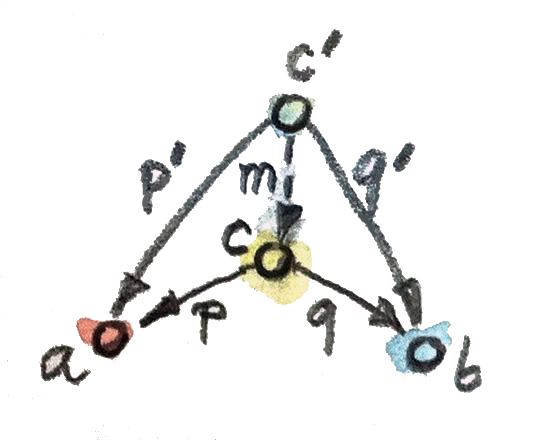
\includegraphics[width=1.78125in]{images/productranking.jpg}

A product is a special case of a limit. A limit is defined in terms of
cones. A general cone is built from commuting diagrams. Commutativity of
those diagrams may be replaced with a suitable naturality condition for
the mapping of functors. This way commutativity is reduced to the role
of the assembly language for the higher level language of natural
transformations.

\subsection{Natural Transformations}\label{natural-transformations}

In general, natural transformations are very convenient whenever we need
a mapping from morphisms to commuting squares. Two opposing sides of a
naturality square are the mappings of some morphism \texttt{f} under two
functors \texttt{F} and \texttt{G}. The other sides are the components
of the natural transformation (which are also morphisms).

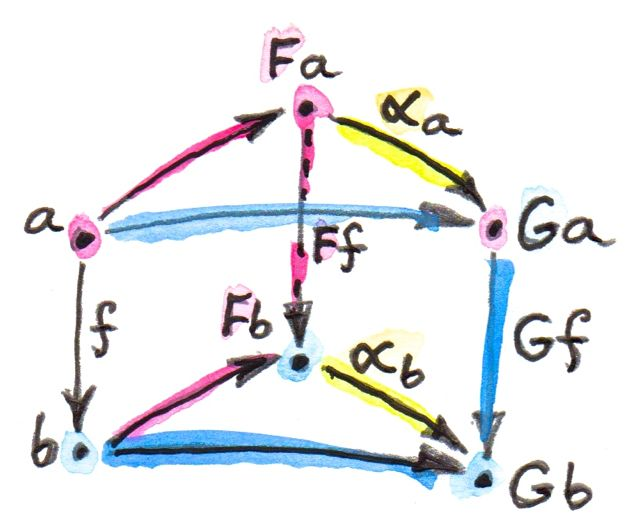
\includegraphics[width=2.25000in]{images/3_naturality.jpg}

Naturality means that when you move to the ``neighboring'' component (by
neighboring I mean connected by a morphism), you're not going against
the structure of either the category or the functors. It doesn't matter
whether you first use a component of the natural transformation to
bridge the gap between objects, and then jump to its neighbor using the
functor; or the other way around. The two directions are orthogonal. A
natural transformation moves you left and right, and the functors move
you up and down or back and forth --- so to speak. You can visualize the
\emph{image} of a functor as a sheet in the target category. A natural
transformation maps one such sheet corresponding to F, to another,
corresponding to G.

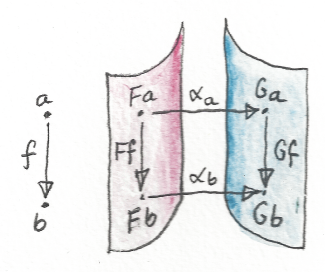
\includegraphics{images/sheets.png}

We've seen examples of this orthogonality in Haskell. There the action
of a functor modifies the content of a container without changing its
shape, while a natural transformation repackages the untouched contents
into a different container. The order of these operations doesn't
matter.

We've seen the cones in the definition of a limit replaced by natural
transformations. Naturality ensures that the sides of every cone
commute. Still, a limit is defined in terms of mappings \emph{between}
cones. These mappings must also satisfy commutativity conditions. (For
instance, the triangles in the definition of the product must commute.)

These conditions, too, may be replaced by naturality. You may recall
that the \emph{universal} cone, or the limit, is defined as a natural
transformation between the (contravariant) hom-functor:

\begin{verbatim}
F :: c -> C(c, Lim D)
\end{verbatim}

and the (also contravariant) functor that maps objects in \emph{C} to
cones, which themselves are natural transformations:

\begin{verbatim}
G :: c -> Nat(Δc, D)
\end{verbatim}

Here, \texttt{Δc} is the constant functor, and \texttt{D} is the functor
that defines the diagram in \emph{C}. Both functors \texttt{F} and
\texttt{G} have well defined actions on morphisms in \emph{C}. It so
happens that this particular natural transformation between \texttt{F}
and \texttt{G} is an \emph{isomorphism}.

\subsection{Natural Isomorphisms}\label{natural-isomorphisms}

A natural isomorphism --- which is a natural transformation whose every
component is reversible --- is category theory's way of saying that
``two things are the same.'' A component of such a transformation must
be an isomorphism between objects --- a morphism that has the inverse.
If you visualize functor images as sheets, a natural isomorphism is a
one-to-one invertible mapping between those sheets.

\subsection{Hom-Sets}\label{hom-sets}

But what are morphisms? They do have more structure than objects: unlike
objects, morphisms have two ends. But if you fix the source and the
target objects, the morphisms between the two form a boring set (at
least for locally small categories). We can give elements of this set
names like \texttt{f} or \texttt{g}, to distinguish one from another ---
but what is it, really, that makes them different?

The essential difference between morphisms in a given hom-set lies in
the way they compose with other morphisms (from abutting hom-sets). If
there is a morphism \texttt{h} whose composition (either pre- or post-)
with \texttt{f} is different than that with \texttt{g}, for instance:

\begin{verbatim}
h ∘ f ≠ h ∘ g
\end{verbatim}

then we can directly ``observe'' the difference between \texttt{f} and
\texttt{g}. But even if the difference is not directly observable, we
might use functors to zoom in on the hom-set. A functor \texttt{F} may
map the two morphisms to distinct morphisms:

\begin{verbatim}
F f ≠ F g
\end{verbatim}

in a richer category, where the abutting hom-sets provide more
resolution, e.g.,

\begin{verbatim}
h&apos; ∘ F f ≠ h&apos; ∘ F g
\end{verbatim}

where \texttt{h\&apos;} is not in the image of \texttt{F}.

\subsection{Hom-Set Isomorphisms}\label{hom-set-isomorphisms}

A lot of categorical constructions rely on isomorphisms between
hom-sets. But since hom-sets are just sets, a plain isomorphism between
them doesn't tell you much. For finite sets, an isomorphism just says
that they have the same number of elements. If the sets are infinite,
their cardinality must be the same. But any meaningful isomorphism of
hom-sets must take into account composition. And composition involves
more than one hom-set. We need to define isomorphisms that span whole
collections of hom-sets, and we need to impose some compatibility
conditions that interoperate with composition. And a \emph{natural}
isomorphism fits the bill exactly.

But what's a natural isomorphism of hom-sets? Naturality is a property
of mappings between functors, not sets. So we are really talking about a
natural isomorphism between hom-set-valued functors. These functors are
more than just set-valued functors. Their action on morphisms is induced
by the appropriate hom-functors. Morphisms are canonically mapped by
hom-functors using either pre- or post-composition (depending on the
covariance of the functor).

The Yoneda embedding is one example of such an isomorphism. It maps
hom-sets in \emph{C} to hom-sets in the functor category; and it's
natural. One functor in the Yoneda embedding is the hom-functor in
\emph{C} and the other maps objects to sets of natural transformations
between hom-sets.

The definition of a limit is also a natural isomorphism between hom-sets
(the second one, again, in the functor category):

\begin{verbatim}
C(c, Lim D) ≃ Nat(Δc, D)
\end{verbatim}

It turns out that our construction of an exponential object, or that of
a free monoid, can also be rewritten as a natural isomorphism between
hom-sets.

This is no coincidence --- we'll see next that these are just different
examples of adjunctions, which are defined as natural isomorphisms of
hom-sets.

\subsection{Asymmetry of Hom-Sets}\label{asymmetry-of-hom-sets}

There is one more observation that will help us understand adjunctions.
Hom-sets are, in general, not symmetric. A hom-set \texttt{C(a,\ b)} is
often very different from the hom-set \texttt{C(b,\ a)}. The ultimate
demonstration of this asymmetry is a partial order viewed as a category.
In a partial order, a morphism from \texttt{a} to \texttt{b} exists if
and only if \texttt{a} is less than or equal to \texttt{b}. If
\texttt{a} and \texttt{b} are different, then there can be no morphism
going the other way, from \texttt{b} to \texttt{a}. So if the hom-set
\texttt{C(a,\ b)} is non-empty, which in this case means it's a
singleton set, then \texttt{C(b,\ a)} must be empty, unless
\texttt{a\ =\ b}. The arrows in this category have a definite flow in
one direction.

A preorder, which is based on a relation that's not necessarily
antisymmetric, is also ``mostly'' directional, except for occasional
cycles. It's convenient to think of an arbitrary category as a
generalization of a preoder.

A preorder is a thin category --- all hom-sets are either singletons or
empty. We can visualize a general category as a ``thick'' preorder.

\subsection{Challenges}\label{challenges}

\begin{enumerate}
\tightlist
\item
  Consider some degenerate cases of a naturality condition and draw the
  appropriate diagrams. For instance, what happens if either functor
  \texttt{F} or \texttt{G} map both objects \texttt{a} and \texttt{b}
  (the ends of \texttt{f\ ::\ a\ -\textgreater{}\ b}) to the same
  object, e.g., \texttt{F\ a\ =\ F\ b} or \texttt{G\ a\ =\ G\ b}?
  (Notice that you get a cone or a co-cone this way.) Then consider
  cases where either \texttt{F\ a\ =\ G\ a} or \texttt{F\ b\ =\ G\ b}.
  Finally, what if you start with a morphism that loops on itself ---
  \texttt{f\ ::\ a\ -\textgreater{}\ a}?
\end{enumerate}

Next:
\href{https://bartoszmilewski.com/2016/04/18/adjunctions/}{Adjunctions}.

\subsection{Acknowledgments}\label{acknowledgments}

I'd like to thank Gershom Bazerman for checking my math and logic, and
André van Meulebrouck, who has been volunteering his editing help
throughout this series of posts.\\
\href{https://twitter.com/BartoszMilewski}{Follow @BartoszMilewski}
